%*******************************************************************************
%****************************** Fourth Chapter *********************************
%*******************************************************************************

\chapter{Evaluation}

\ifpdf
    \graphicspath{image/}
\fi

This section discusses the performance of each LSB-pair methods by using three image quality measurement approaches: Peak signal-to-noise ratio (PSNR), Histogram absolute error (Hae) and Structural similarity index measure (SSIM). In our experiment, we used an image set which came from GHIM-10K  ~\cite{liu2015content} and it contains ten thousand images. In this image set, all images are grayscale images which is either $400 \times 300$ or $300 \times 400$ in resolution. The embedding message is 6,219 English characters in length and encoded with ASCII code standard, 1 byte for each character. We embedded this 6,219 bytes size message into these grayscale images using five LSB embed methods: original LSB replacement, LSB-pair, LSB-crossline-pair, LSB-triple-pair and LSB-combine-pair. 

Before comparing the performance of these methods, one thing that needs to be mentioned is that the error rate of extracting watermarked message by using these methods is 0\% over these 10,000 images. For digital watermarking, the robustness is one of the core requirements. This experiment result shows that these methods are stable and reliable enough to be considered as new methods in digital watermarking field.

\section{\label{sec:level1}Hae}

Histogram absolute error (Hae) is a method which intuitively indicates the total difference between original image and watermarked image. In the previous section we had defined the distortion distribution of gray level pixels is: \(D = (d_{0}, d_{1}, d_{2} … , d_{253}, d_{254}, d_{255})\); the distortion changes between watermarked image and original image is: \(D' = D_{2} - D_{1}, D' = (d'_{0}, d'_{1}, d'_{2} … , d'_{253}, d'_{254}, d'_{255})\). Yang ~\cite{ren2014image} used a formula to calculate histogram absolute error:
$$h(n) = \sum_{i=1}^{H}*\sum_{j=1}^{W}(\delta(n,P(i,j)))$$

where
$$\delta(u,v) = \begin{cases} 1, & u = v \\ 
0, & u \neq v \end{cases}$$

In his formula, H and W is the height and width of the carrier image respectively. P(i,j) is the gray level of a special pixel, in this thesis, it is the same as \(G(P_{i})\) which also refer to the gray level of  pixel \(P_{i}\). The element \textit{n} represents the gray intensity value, for example, in an 8 bits per pixel image, \(n \in [0,255]\) and \(n\in N\). \(255\) comes from \(2^{8} -1\) which is the maximum value of gray level. According to the previous image distortion definition and the image set we used, this formula can be simplified to:

$$h(n) = \sum_{i=1}^{255} d_{i}$$

Then calculate distortion change:
$$Hae = \sum_{i=1}^{255} (d2_{i} - d1_{i}) = \sum_{i=1}^{255} d'_{i}$$

Form the definition, the value of Hae smaller than 0 represents distortion have reduced, vise verse. FIG 4.1 shows the pseudocode of this method.

\begin{figure}[h]
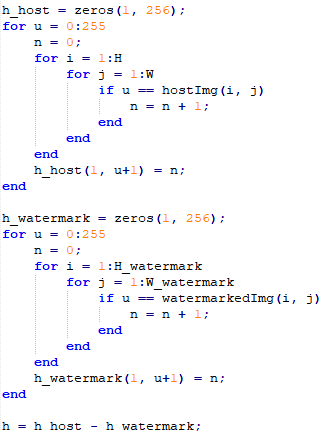
\includegraphics[width=\columnwidth]{image/Pseudocode_Hae.PNG}
\caption{Pseudocode of Hae}
\label{fig:figure}
\end{figure}   



\section{\label{sec:level1}PSNR}

Peak signal-to-noise ratio (PSNR) is one of the most  important and commonly used measurements to evaluate image quality. PSNR is an engineering term for the ratio between the maximum possible power of a signal and the power of corrupting noise that affects the fidelity of its representation. MSE is mean squared error between two images. The higher value of MES represents higher error as well as the worse picture quality ~\cite{eratne2009fast}.

The formula of PSNR is:

\begin{align*}  
PSNR    &=  10* \log_{10} \frac{MAX^2_{1}}{MSE} \\
        &=  20 *\log_{10} \frac{MAX_{1}}{\sqrt{MSE}}
\end{align*} 

which the formula of MSE is:

$$MSE = \frac{1}{mn}\sum_{i=0}^{m-1}\sum_{j=0}^{n-1} [I(i,j)-K(i,j)]^2$$

In PSNR formula, the MAX means the maximum possible value of the image. For example, if there is a picture which is 8 bits per pixel, the maximum value is 255, if it is14 bits, the MAX in this situation is 16383. As for a colourful picture, there has three MSE values corresponding to Red, Green and Blue, and there have three PSNR values for each colour as well. Which means, a colourful image has a vector of three PSNR values to evaluate its quality.


Generally, for PSNR, 30 to 50 dB noise for 8 bits picture, 60 to 80 dB noise for 16bits picture are considered as an acceptable image quality changes. However, PSNR is not friendly for human vision. The value of PSNR is not exactly how we humans think. Because it just uses mean square value to evaluate image, does not consider the image inside, which means, it does not care about what this image is, just evaluate the total and average value or energy changes of these two images.

However, this image quality measurement does not take into account how human's visual system perceives images, which itself may be different for different individuals. It is very complex and cannot be treated as a linear system; the result of human vision evaluation can be influenced by individual’s background, knowledge and motivation. The observation environment is also a significant parameter ~\cite{Tong2006IamgeQuality}. Tong ~\cite{Tong2006IamgeQuality} used FIG 4.2 as an example in his paper. The image in middle is the original image, it is obvious that most people think the left one is more similar than the right one. However, these two have the same PSNR value. For this reason, our experiment only uses PSNR as a reference measurement approach, instead of treating it as a core indicator for image changes.

\begin{figure}[h]
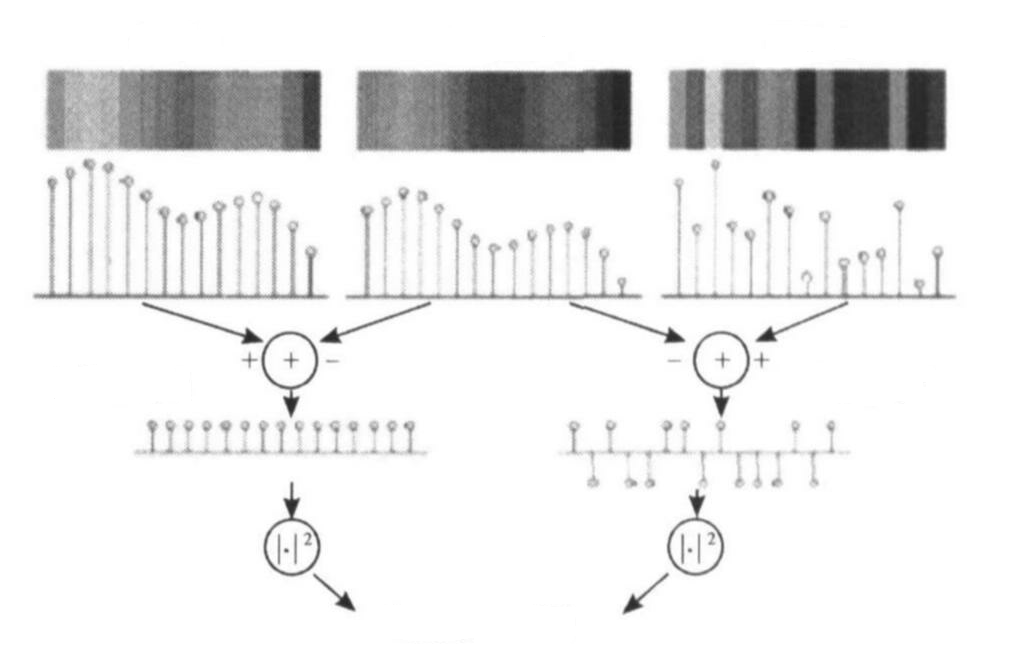
\includegraphics[width=\columnwidth]{image/PSNR_example.png}
\caption{PSNR example \cite{Tong2006IamgeQuality}}
\label{fig:figure}
\end{figure} 


\section{\label{sec:level1}SSIM}

Structural similarity index measure (SSIM) performs well for static image measure. Regular approaches are going to solve absolute errors, however, SSIM is perception-based model which can consider image degradation. Image degradation is considered as a perceived change in the structural information of the image.  It not only considers the RGB (Red, Blue, Green) colour channels, but also YUV (Luminance, Chrominance, Chroma). This approach believes each pixel have strong inter-dependencies especially when they are spatially close.

According to Wang’s research, SSIM has better performance than PSNR but it requires more computing power and processing time to measurement two images. However, it does not totally solve the weaknesses of PSNR. ~\cite{wang2005structural} The algorithm for SSIM is complex, generally, it separates image to various windows and measure between windows. The formula is:

\begin{equation}
SSIM ( f ,g ) = l ( f ,g )c ( f ,g )s ( f ,g )
\end{equation}

\begin{equation}
\begin{cases} l(f,g) = \frac{2\mu_{f}\mu_{g} + C_{1}}{\mu^2_{f} + \mu^2_{g} + C_{1}}\\ 
c(f,g) = \frac{2\sigma_{f}\sigma_{g} + C_{2}}{\sigma^2_{f} + \sigma^2_{g} + C_{2}}\\
s(f,g) = \frac{\sigma_{fg} + C_{3}}{\sigma_{f}\sigma_{g} + C_{3}}
\end{cases}
\end{equation}


The first term in (4.2) is the luminance comparison function which measures the closeness of the two images’ mean luminance \((\mu_{f}\)  and \(\mu_{g})\). c(f,g) is the function of measure contrast comparison, and the third item is for the structure comparison. \(C_{1}\), \(C_{2}\) and \(C_{3}\) is positive constants which are used to provide from null denominator.


\section{\label{sec:level1}Experiment and results}

This section discusses the results of original LSB replacement and four LSB-pair methods using three image quality measurement approaches mentioned in the previous sections. This section goes through one image quality measurement approach by another and compares each LSB method to confirm which method have the best performance for this metric.  

As outlined in the methodology, experiments were done in MATLAB. One grayscale image produces one output image for each of the LSB methods. After embedding messages, the code compares the output images with their original images, then we generate an excel document to display the result.

FIG 4.3 shows the digital watermarked image which is embedded with information invisibly, (a) is the original $512 \times 512$ carrier image. Image (b), (c), (d), (e), (f) are done by original LSB replacement, LSB-pair, LSB-crossline-pair, LSB-triple-pair, LSB-combine-pair respectively. 


% \begin{figure}[h]
% 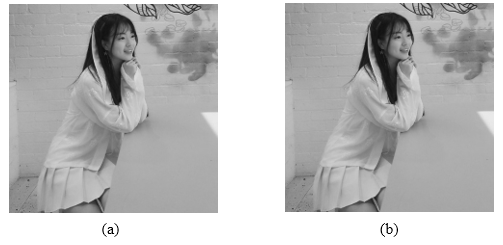
\includegraphics[width=\columnwidth]{image/ab.PNG}
% \label{fig:figure}
% \end{figure} 

% \begin{figure}[h]
% 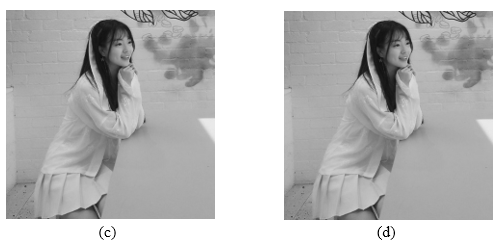
\includegraphics[width=\columnwidth]{image/cd.PNG}
% \label{fig:figure}
% \end{figure} 

% \begin{figure}[h]
% 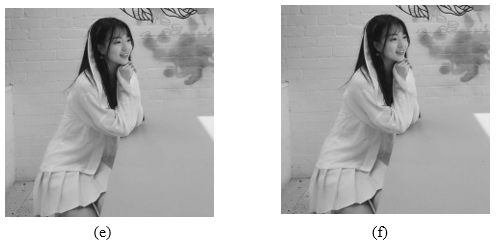
\includegraphics[width=\columnwidth]{image/ef.PNG}
% \caption{Watermarking embedding}
% \label{fig:figure}
% \end{figure} 

\begin{figure}[h]
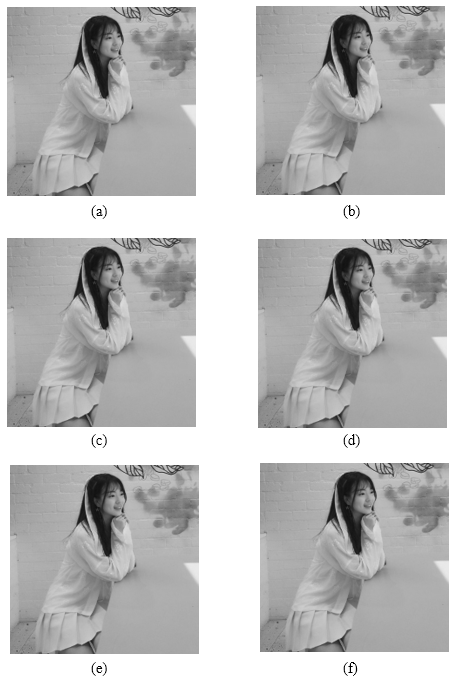
\includegraphics[width=\columnwidth]{image/abcdef.PNG}
\caption{Watermarking embedding}
\label{fig:figure}
\end{figure} 


FIG 4.4 and Table 4.1 show the PSNR results for the regular LSB replacement, LSB-pair, LSB-crossline-pair, LSB-triple-pair and LSB-combine-pair. From the table, it is clear that all these methods have the same PSNR value. These results are the same as our expectation. According to these LSB-pair methods embedding mechanism, it is not hard to prove they have same PSNR value. Here is a prove of original LSB replacement and LSB-pair having same PSNR value: 

\begin{itemize}
  \item If two adjacent pixels are not a pair, they need to be applied for original LSB replacement, hence, the PSNR not change when two pixels are not a pair.
  \item Assuming \(P_{i}, P_{i+1}\) meets LSB pair requirements, \(P_{i} = P_{i+1} + 1\) and \(LSB(P_{i}) = 0\), from the definition, we have \(M_{i} = 1, M_{i+1} = 0\).
  \item If we use original LSB replacement, the embedded pixel \(P'_{i} = P_{i} + 1\), \(P'_{i+1} = P_{i+1} - 1\), \(LSB(P'_{i}) = 1, LSB(P'_{i+1}) = 0\). In this case, calculate MSE difference for these two pixels: \((P'_{i} - P_{i})^2 + (P'_{i+1} - P_{i+1})^2 = 1 + 1 = 2\)
  \item If we use LSB-pair, swaping \(P_{i}\) and \(P_{i+1}\) at first, get \(P'_{i} = P_{i+1} = P_{i} - 1, P'_{i+1} = P_{i} = P_{i+1} + 1\). In this case, calculate MSE difference for these two pixels: \((P'_{i} - P_{i})^2 + (P'_{i+1} - P_{i+1})^2 = 1 + 1 = 2\). Therefore, the PSNR does not change compared with using original LSB replacement.
  \item The same derivation process for the situation \(P_{i} = P_{i+1} - 1, M_{i} = 0, M_{i+1} = 1\).
\end{itemize}

      
To sum up, this proof can be extended to other LSB-pair extension methods,  to prove that original LSB replacement method has the same PSNR value with others LSB-pair variation methods. Due to this phenomenon, PSNR  is not a reliable image quality measurement approach in this situation. However, it can be a verification method to check if the message is correctly embedded or not.


Table 4.1 shows the average, maximum and minimum PSNR value in this image set. Form the PSNR definition, 1 to 5 dB change is an acceptable image change. Therefore, we can conclude that the LSB-pair methods will not change the carrier image significantly and these methods have the capacity to embed the message invisibly in PSNR level.

\begin{table*}
\begin{tabular}{ |c|c|c|c|  }
 \hline
 \multicolumn{4}{|c|}{PSNR(dB)} \\
 \hline
 LSB methods        &Mean           &Maximum        &Minimum\\
 \hline
 LSB                &1.743856156    &4.247659738    &0.33989157\\
 \hline
 LSB-pair           &1.743856156	&4.247659738	&0.33989157\\
 \hline
 LSB-crossline-pair &1.743856156    &4.247659738    &0.33989157\\
 \hline
 LSB-triple-pair    &1.743856156    &4.247659738    &0.33989157\\
 \hline
 LSB-combine-pair   &1.743856156    &4.247659738    &0.33989157\\
 \hline
\end{tabular}
 \caption{Summary of PSNR}
\end{table*}

\begin{figure}[h]
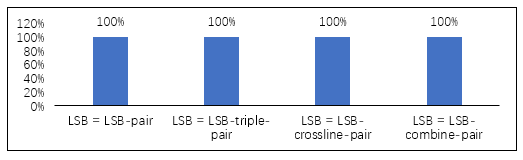
\includegraphics[width=\columnwidth]{image/PSNR.PNG}
\caption{PSNR result}
\label{fig:figure}
\end{figure} 


FIG 4.5  shows the experiment result for using Hae. This approach calculates the gray level difference between original image and watermarked image. If the Hae value difference is lower than 0, it means the distortion is reduced. In this histogram, better means the first embedding method has better distortion reducing performance than the second method. In other word, the better in the histogram represents Haefirst method – Haesecond method < 0.

Comparing application of original LSB replacement with others, an average of 6\% of the images have better distortion reduction than other four LSB-pair methods. LSB-pair takes the lowest at 5.18\%, and LSB-combine-pair is the highest at 6.96\%. As for better Hae value comparing with original LSB replacement, LSB-pair performs worst. Original LSB replacement has 24.53\% of images having higher distortion than using LSB-pair. In contrast, LSB-combine-pair performs the best -- 31.28\% have lower distortion than applying original LSB replacement method. However, the most number of image sets have the same distortion, they occupy about 60-70\%. 

As for comparison of LSB-pair and its variations methods using Hae measurement approach, the result generally looks the same -- about 70\% images have the same Hae value. Nonetheless, when looking at this result in more detail, the features of each method are different. Extension LSB-pair methods (LSB-crossline-pair, LSB-triple-pair, LSB-combine-pair) all have a higher percentage of reducing distortion rather than increasing distortion compared with regular LSB replacement. LSB-crossline-pair performs better than LSB-triple-pair: 18.03\% of images have lower distortion than applying LSB-triple-pair and 9.96\% images have higher distortion, and the rest have the same distortion. 
From this data, we can draw a conclusion that, in most cases, LSB-crossline-pair and LSB-triple-pair have similar performances. In the remaining situations, two thirds of images have less distortion change than applying LSB-crossline-pair. Hence, we can conclude that, the LSB-crossline-pair method have better performance than LSB-triple-pair on Hae measurement approach. In LSB-combine-pair, this is the main reason that crossline pair detection has higher priority than jump pixel detection. As for LSB-combine-pair, it performs better than any other methods.

Table 4.2 shows the summary of Hae. It indicates that Hae of original LSB replacement is 0.0224\%, 0.0642\%, 0.0504\%, 0.0834\% higher than LSB-pair, LSB-crossline-pair, LSB-triple-pair, LSB-combine-pair respectively on average. One interesting thing to note is the maximum of Hae is equal across all methods. Tracing back, we find that the image which cause these outlier values is the same one. In this image, it has three unusual features: over 70\% pixels are in the same colour (gray level: 0); pixel gray level changes sharply; there few LSB pairs which can be detected. With the above findings, we can draw a conclusion: a carrier image with complex compositions, variety of colours (gray levels) and no sharp edges in the image is ideal for applying the LSB-pair methods.

\begin{figure}[h]
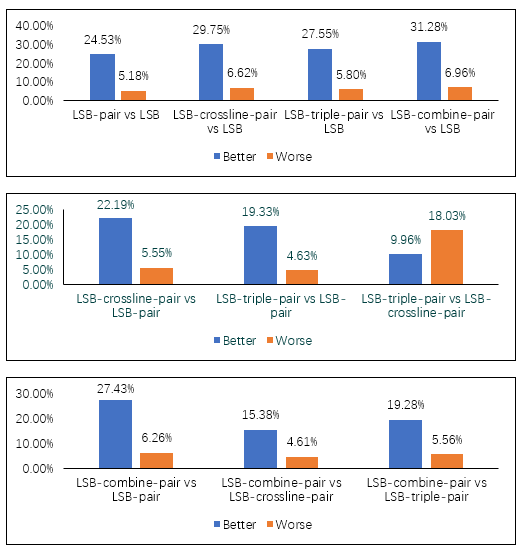
\includegraphics[width=\columnwidth]{image/Hae.PNG}
\caption{Hae result}
\label{fig:figure}
\end{figure} 


\begin{table*}
\centering
\begin{tabular}{|c|c|c|c|c|c|c|}
 \hline
 \multicolumn{7}{|c|}{Histogram absolute error} \\
 \hline
 LSB methods        &Minimum&1st Quartile	&Median	&Mean	    &3rd Quartile	&Maximum\\
 \hline
 LSB&               16950	&42280	        &42868	&43693.44	&43534	        &110376\\
 \hline
 LSB-pair	        &16722	&42274	        &42862	&43683.64	&43526	        &110376\\
 \hline
 LSB-crossline-pair	&16398	&42262	        &42855	&43665.42	&43512	        &110376\\
 \hline
 LSB-triple-pair	&16428	&42268	        &42858	&43671.42	&43518	        &110376\\
 \hline
 LSB-combine-pair	&15832	&42254	        &42851	&43657.03	&43506	        &110376\\
 \hline
\end{tabular}
 \caption{Summary of Hae}
\end{table*}


FIG 12 and table 4.3 indicate the values of using SSIM. Due to the original SSIM value difference is tiny and it is hard for our observation. We use a formula \((1 - SSIM) * 10000\) to zoom in these data. Due to higher SSIM value represents more similar to the original image, in this case, the lower value displayed in the table means the better performance in SSIM. In general, all these extension LSB-pair methods have poorer performance than original LSB replacement. Besides original LSB replacement methods, LSB-triple-pair has the best performance, where 17.19\% of the watermarked images are better than which applying original LSB-replacement; for LSB-pair, this rate is 10.78; 9.81\% for LSB-crossline-pair and 11.56\% for LSB-combine-pair. When comparing LSB-triple-pair with LSB-crossline-pair and LSB-combine-pair, 64.94\% and 89.96\% of images have better SSIM value respectively. 

One thing to note is that LSB-triple-pair has better performance than LSB-pair when compared with original LSB replacement. However, LSB-triple-pair only has 25.55\% of images having better SSIM value than LSB-pair. It means that, if one image applied with LSB-pair method has worse performance than original LSB replacement, it is highly probable that for the same image, LSB-triple-pair may have worse performance than LSB-pair. It also means that for this image, it is very likely that applying LSB-triple-pair yields worse performance than original LSB replacement, and vice versa. As for LSB-combine-pair, it performs the worst in SSIM evaluation; the rates of worse performance are all higher than the rates of better when compared with other methods. However, it does not necessarily mean that LSB-combine-pair is not a suitable digital watermarking embedding method and not friendly to human visual system. Table 4.3 points out that all methods have very narrow gaps with each other, even when the differences have been zoom in ten thousand times. 

\begin{figure}[h]
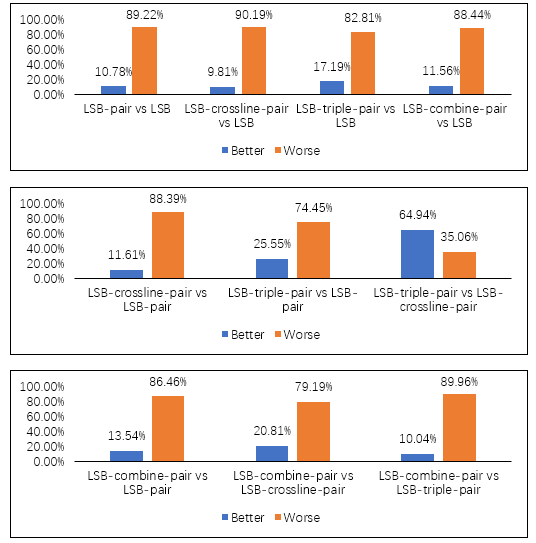
\includegraphics[width=\columnwidth]{image/SSIM.PNG}
\caption{SSIM result}
\label{fig:figure}
\end{figure} 


\begin{table*}
\centering
\begin{tabular}{ |c|c|c|c|c|c|c|  }
 \hline
 \multicolumn{7}{|c|}{(1 - SSIM) * 10000} \\
 \hline
 LSB methods    &Minimum&1st Quartile	&Median	&Mean	&3rd Quartile	        &Maximum\\
 \hline
 LSB	            &2.2705	&20.8321	&27.4459	    &28.8292	&33.5760	&439.2084\\
 \hline
 LSB-pair	        &2.2702	&20.8382	&27.4670	    &28.8401	&33.5981	&439.1730\\
 \hline
 LSB-crossline-pair	&2.2701 &20.8792	&27.5242	    &28.8748	&33.6363	&439.1106\\
 \hline
 LSB-triple-pair	&2.2703	&20.8726	&27.5267	    &28.8617	&33.6324	&438.9516\\
 \hline
 LSB-combine-pair	&2.2700	&20.9028	&27.5861	    &28.8962	&33.6887	&438.9165\\
 \hline
\end{tabular}
 \caption{Summary of SSIM}
\end{table*}


In theory, LSB-crossline-pair has less chances to find pairs than LSB-triple-pair. Because in a \(n \times m\) image, except last two pixels, LSB-triple-pair has \(n \times m -2\) chances of finding a pair. However, LSB-crossline-pair only has \(n \times m - n\) chances, except the pixels that are in the last row. Therefore, if an image is large enough, the method LSB-triple-pair should perform \(1/m\) better than LSB-crossline-pair, because, in theory, it has 1/m more attempts to find pairs. However, the experiment results show that LSB-crossline-pair has better performance in Hae which is against our assumption. 

We suppose this difference is owing to the distance of pixel pair. In FIG 4.7, assuming current pixel is \(P_{7}\), LSB-pair compares it with \(P_{8}\) which has an Euclidean distance of 1; LSB-crossline-pair compares with \(P_{8}\) and \(P_{12}\) which also has Euclidean distance of 1; LSB-triple-pair compares with \(P_{8}\) and \(P_{9}\) with distance of either 1 or 2. Assuming LSB-crossline-pair has better performance in reducing distortion then LSB-triple-pair, we can make a prediction that the lower Euclidean distance will have better performance in LSB-pair extension methods. Therefore, we can predict that LSB-diagonal-pair (\(P_{7}\) with \(P_{8}\) and \(P_{13}\)) has better performance than LSB-crossDoubleLine-pair (\(P_{7}\) with \(P_{8}\) and \(P_{17}\)). However, the additional experiment shows that LSB-crossDoubleLine-pair yields better performance than LSB-diagonal-pair (FIG 4.8 and FIG 4.9). Hence, our previous assumption is invalid. 

In general, there are two shortcomings for the LSB-pair methods: lack of the global view, and pair detection is incomplete for extension methods. In our design, these methods can ensure that the distortion will not increase in each logic iteration when a pixel pair has been found. The fact is, in each logic iteration, the distortion does not increase; however, the Hae experiment results show that there still exist a fair number of distortion increases. This is because these methods do not have an overview of total gray level distribution. For each pixel swapping, distortion can be reduced in this specific logic iteration. Nevertheless, for the whole watermarked image, this iteration of pixel swapping might lead to increase in the total distortion. Another weakness is that the extension methods are incomplete. For example, in LSB-triple-pair, we only find pixel pair between first pixel with second, and first with third. We missed the possibility that the second and the third pixel can make a pair. This is one of the reasons that may explain why LSB-crossLine-pair has better performance than LSB-triple-pair. 


There are no precise rules for selecting which measurement approaches is ideal when the evaluation of image quality is required. The aim of using these approaches is to visualise the distortion changes, which is hard to find out and comparing. PSNR is a measurement which focuses on finding the image energy change for each pixel changes respectively. SSIM is a measurement which is interested in the image structure changes. The Hae is an approach for summing up image pixel gray level distortion. Therefore, from the emphasis of each approaches, the result of Hae is considered as the highest priority in our evaluation. As for PSNR and SSIM, they are considered as assisting evaluation approaches. Their results also need to be pay attention to because they can help to guarantee image quality in an acceptable field after embedding security messages. 

In summary, the performance of distortion reduction sorted from best to worst: LSB-combine-pair>LSB-crossDoubleLine-pair>LSB-diagonal-pair>LSB-crossLine-pair>LSB-triple-pair>LSB-pair.


\begin{figure}[h]
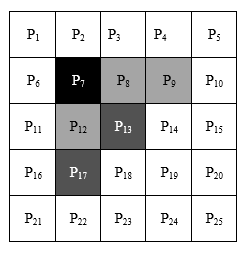
\includegraphics[width=\columnwidth]{image/Euclidean_distance.PNG}
\caption{Euclidean distance}
\label{fig:figure}
\end{figure} 

\begin{figure}[h]
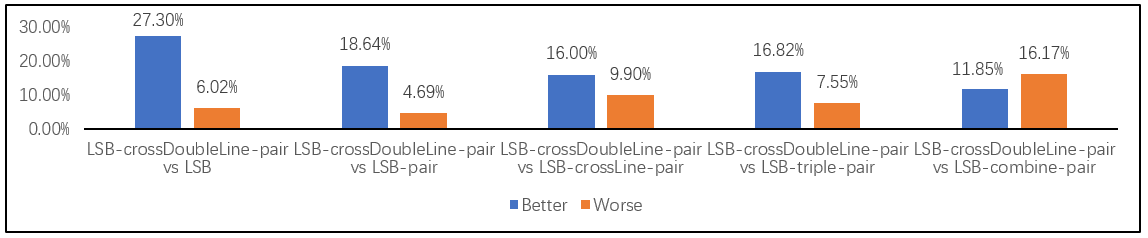
\includegraphics[width=\columnwidth]{image/LSB-crossDoubleLine-pair.PNG}
\caption{Hea for LSB-crossDoubleLine-pair}
\label{fig:figure}
\end{figure} 

\begin{figure}[h]
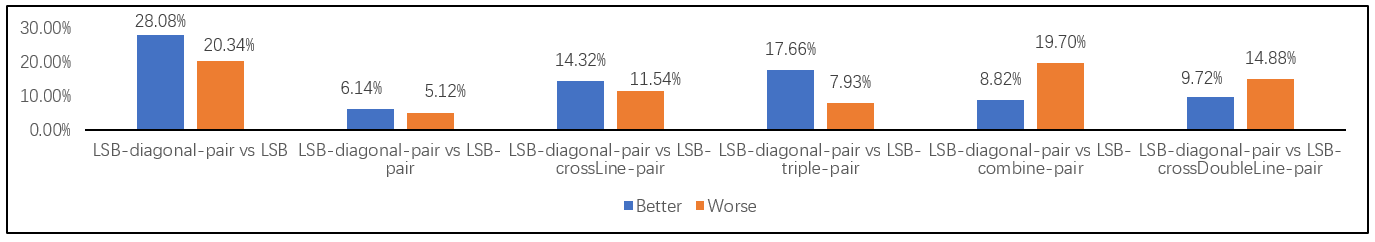
\includegraphics[width=\columnwidth]{image/LSB-diagonal-pair.PNG}
\caption{Hea for LSB-diagonal-pair}
\label{fig:figure}
\end{figure} 
